%% LaTeX Beamer presentation template (requires beamer package)
%% see http://bitbucket.org/rivanvx/beamer/wiki/Home
%% idea contributed by H. Turgut Uyar
%% template based on a template by Till Tantau
%% this template is still evolving - it might differ in future releases!

\documentclass{beamer}

\mode<presentation>
{
\usetheme{Berlin}

\setbeamercovered{transparent}
\setbeamertemplate{footline}[frame number]
\beamertemplatenavigationsymbolsempty

}

\newcommand{\RM}[1]{\MakeUppercase{\romannumeral #1{}}}

\usepackage[ngerman]{babel}
\usepackage[utf8]{inputenc}

% font definitions, try \usepackage{ae} instead of the following
% three lines if you don't like this look
\usepackage{mathptmx}
\usepackage{lmodern}
%\usepackage[scaled=.90]{helvet}
%\usepackage{courier}

\usepackage[T1]{fontenc}

\usepackage{listings}
\usepackage{color}

\definecolor{javared}{rgb}{0.6,0,0} % for strings
\definecolor{javagreen}{rgb}{0.25,0.5,0.35} % comments
\definecolor{javapurple}{rgb}{0.5,0,0.35} % keywords
\definecolor{javadocblue}{rgb}{0.25,0.35,0.75} % javadoc
 
\lstdefinestyle{mystyle}{
    backgroundcolor=\color{white},   
    commentstyle=\color{javagreen},
    keywordstyle=\color{javapurple},
    stringstyle=\color{javared},
    rulecolor=\color{black},
    basicstyle=\footnotesize,
    breakatwhitespace=false,         
    breaklines=true,                 
    captionpos=b,                    
    keepspaces=true,                 
    numbers=none,                    
    numbersep=5pt,                  
    showspaces=false,                
    showstringspaces=false,
    showtabs=false,                  
    tabsize=2,
    framerule= 0.1pt,
    frame=tb,
    framextopmargin=6pt,
    framexbottommargin=6pt,
    aboveskip=24pt,
    xleftmargin=0pt,
    numbersep=12pt
}
 
\lstset{style=mystyle}
\lstset{literate=%
    {Ö}{{\"O}}1
    {Ä}{{\"A}}1
    {Ü}{{\"U}}1
    {ß}{{\ss}}1
    {ü}{{\"u}}1
    {ä}{{\"a}}1
    {ö}{{\"o}}1
    {~}{{\textasciitilde}}1
}

\title[]{Entwurf und Implementierung einer prototypischen Webanwendung
					zur Verfügbarmachung personalisierter Inhalte aus einem Content
					Management System via iBeacons}

%\subtitle{}

% - Use the \inst{?} command only if the authors have different
%   affiliation.
%\author{F.~Author\inst{1} \and S.~Another\inst{2}}
\author{Steven Maasch}

% - Use the \inst command only if there are several affiliations.
% - Keep it simple, no one is interested in your street address.
\institute[Beuth Hochschule für Technik Berlin]
{
Fachbereich \RM{6} $\cdot$ Informatik und Medien\\
Studiengang Medieninformatik (BA)\\
Beuth Hochschule für Technik Berlin
}

\date{Berlin, 11. Dezember 2014}

% This is only inserted into the PDF information catalog. Can be left
% out.
\subject{Talks}

% If you have a file called "university-logo-filename.xxx", where xxx
% is a graphic format that can be processed by latex or pdflatex,
% resp., then you can add a logo as follows:

% \pgfdeclareimage[height=0.5cm]{university-logo}{university-logo-filename}
% \logo{\pgfuseimage{university-logo}}



% Delete this, if you do not want the table of contents to pop up at
% the beginning of each subsection:
%\AtBeginSubsection[]
%{
%\begin{frame}<beamer>
%\frametitle{Outline}
%\tableofcontents[currentsection,currentsubsection]
%\end{frame}
%}

% If you wish to uncover everything in a step-wise fashion, uncomment
% the following command:

%\beamerdefaultoverlayspecification{<+->}

\setbeamertemplate{section page}
{
    \begin{centering}

    \begin{beamercolorbox}[sep=12pt,center]{part title}
    \usebeamerfont{section title}\insertsection\par
    \end{beamercolorbox}
    \end{centering}
}

\AtBeginSection{\frame{\sectionpage}}

\begin{document}


\begin{frame}
\titlepage
\end{frame}

\begin{frame}
\frametitle{Gliederung}
\tableofcontents
% You might wish to add the option [pausesections]
\end{frame}

\section{Einleitung}

\begin{frame}

\frametitle{Problemstellung}

\begin{itemize}
  \item Informationsmenge im Internet
  \begin{itemize}
    \item Content-Management-Systeme
    \item Personalisierung von Inhalten
    \end{itemize}
\end{itemize}

\begin{itemize}
 	\item Mobile Endgeräte
	\begin{itemize}
	  \item örtlicher Kontext (Wann und Wo) ist dynamisch
	  \item erschwert Personalisierung
	\end{itemize}
\end{itemize}	
	\begin{itemize}
	  \item Bestimmung des örtlichen Kontextes
	  \begin{itemize}
	  \item GPS, WLAN, IP
	  \item iBeacon
		\end{itemize}
	\end{itemize}

{\textbf{Problem}}

	\begin{itemize}
	  \item keine Integrationsmöglichkeiten
	  \item keine Personalisierung
	\end{itemize}

\end{frame}

\begin{frame}
\frametitle{Ziele der Arbeit}

Prototypische \alert{Erweiterung} des Content-Management-Systems
\alert{FirstSpirit} um folgende \alert{drei Funktionalitäten}:

\begin{enumerate}
	\item Beacon-Management-System
 	\item Verknüpfung von Inhalten mit Beacons
 	\item Schnittstelle zur Personalisierungskomponente
\end{enumerate}

\end{frame}

\section[Hintergrund]{Hintergrund}

\begin{frame}
\frametitle<presentation>{Personalisierung}

{\textbf{Terminologie}}

\begin{itemize}
  \item Anzeige von Inhalten abgestimmt auf jeweiligen Benutzer
  \item basiert auf sog. Benutzerprofilen
  \item Benutzerprofile $\Rightarrow$ Nutzungskontextes ("`W-Fragen"')
  \item Fokussierung auf örtlichen Kontext (Wann und Wo)
\end{itemize}

%\vskip0pt plus.5fill

{\textbf{Personalisierungstechniken}}

\begin{itemize}
  \item Regelbasiertes Filtern
  \item Kollaboratives Filtern
  \item Inhaltsbasiertes Filtern
\end{itemize}

\end{frame}

\begin{frame}
\frametitle<presentation>{Content-Management-Systeme}

\textbf{Zentrale Begriffe}

\begin{definition}[Content]
Als \textit{Content} (dt. Inhalt) bezeichnet man \alert{digitale Daten}, die
  \alert{in Form einer Webseite über} das \alert{Internet verfügbar} sind.
\end{definition}

\begin{definition}[Content-Management-System]
  Ein \textit{Content-Management-System (CMS)} ist ein
  \alert{Softwaresystem} für die \alert{Verwaltung und Administration von Content}.
\end{definition}

\end{frame}

\begin{frame}
\frametitle<presentation>{Content-Management-Systeme}

\textbf{Allgemeiner Aufbau}

\begin{itemize}
  \item Redaktionssystem
  \item Content-Repository
  \item Publishing System
\end{itemize}

\textbf{Systemarchitekturen}

\begin{itemize}
  \item Live-Server-Systeme (dynamisch)
  \item Staging-Server-Systeme (statisch)
\end{itemize}

\textbf{FirstSpirit}

\begin{itemize}
  \item kommerzielles Enterpise-Content-Management-System
  \item basiert auf einer klassischen Client-Server-Architektur
  \item statisches CMS (Staging-Server-System)
  \item vollständig in Java implementiert
  \item eigene Template-Sprache
\end{itemize}

\end{frame}

\begin{frame}
\frametitle<presentation>{iBeacon}

\textbf{Technologie iBeacon}

\begin{itemize}
  \item 2013 von Apple eingeführt
  \item basiert auf Bluetooth-Low-Energy (BLE)
  \item Positionsbestimmung relativ sog. Beacons
\end{itemize}

\textbf{Beacon}

  \begin{itemize}
  \item kleine BLE-Sender
  \item Beacon-Paket (UUID, Major und Minor)
  \item Preis: 20 - 40 Euro 
\end{itemize}

\end{frame}

\section{Anforderungen}

\begin{frame}
\frametitle<presentation>{Zielbestimmung}

  \textbf{Gesamtsystem}
  \begin{itemize}
    \item Bereitstellung von \alert{personalisierten Inhalten} in einem
  bestimmten örtlichen Kontext
  \item Bestimmung des Kontextes mittels \alert{iBeacon}
  \item Darstellung der Inhalte auf \alert{Smartphone}
  \item konkreter Anwendungsfall: \alert{Bücherregal}
  \end{itemize}

\vskip0pt plus.5fill

\textbf{Teilsystem}

\begin{itemize}
  \item Verwaltung von Beacons und Inhalten sowie deren Verknüpfung über das CMS
  FirstSpirit
  \item Externe Verfügbarmachung dieser Daten (Schnittstelle)
\end{itemize}

\end{frame}

\begin{frame}
\frametitle<presentation>{Funktionsübersicht}

\begin{figure}[!h]
\centering
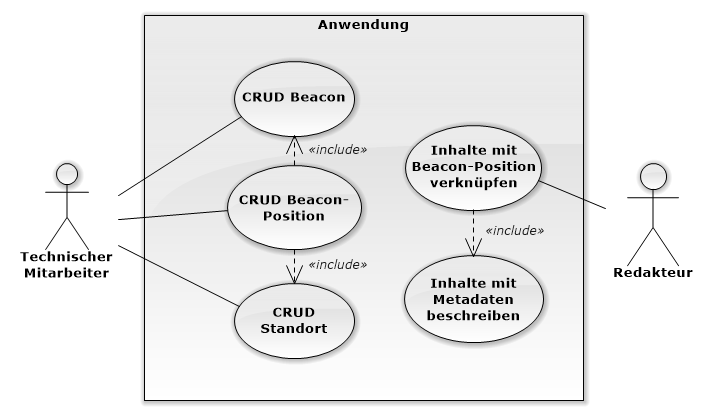
\includegraphics[scale=0.55]{./Abbildungen/Classdiagram2.png}
\label{fig:usecasediagram}
\end{figure}

\end{frame}

% Architektur

\section{Architektur}

\begin{frame}
\frametitle<presentation>{Komponentenmodell}

\begin{figure}[!h]
\centering
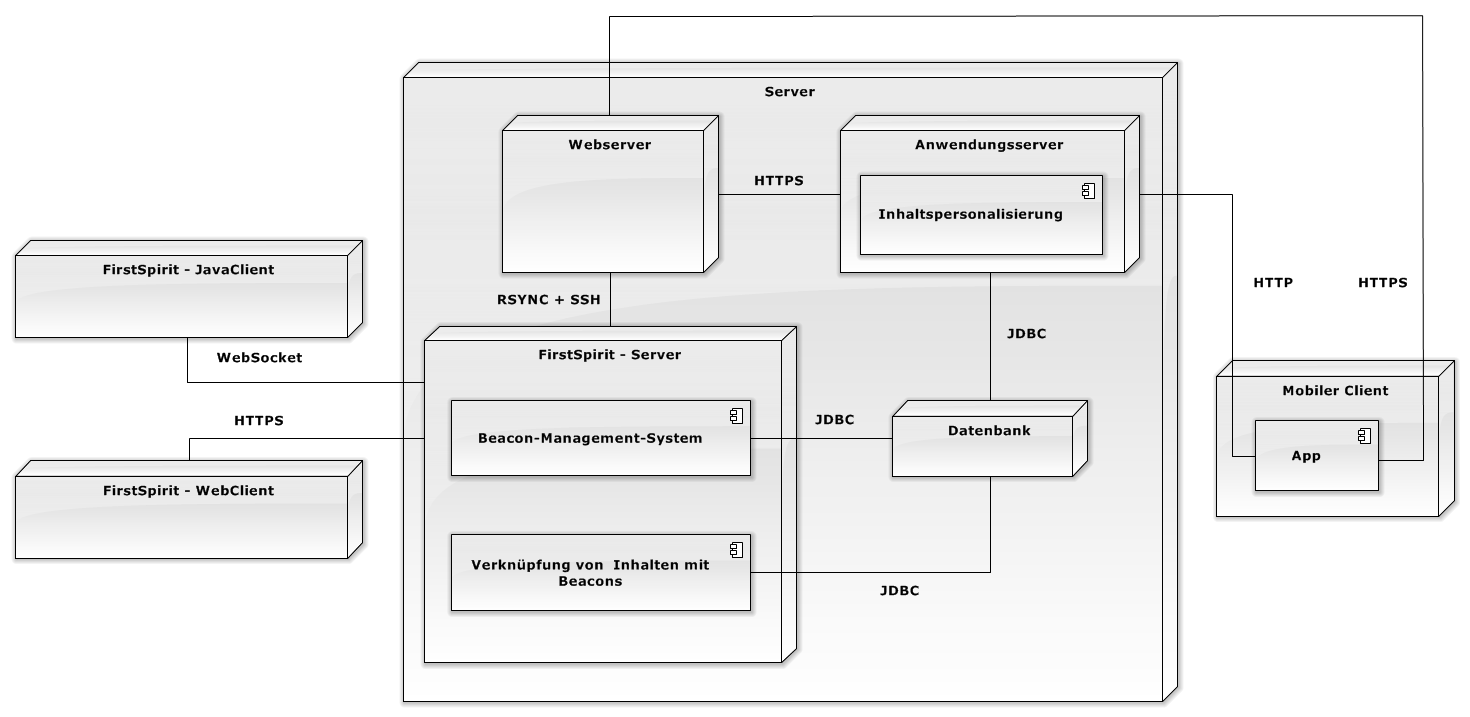
\includegraphics[scale=0.3]{./Abbildungen/Deploymentdiagram2.png}
\end{figure}


\end{frame}

\begin{frame}
\frametitle<presentation>{Systemkomponenten}

\textbf{Software}

 \begin{itemize}
	  		\item Webserver $\Rightarrow$ Apache HTTP Server
	  		\item "`Anwendungsserver"' $\Rightarrow$ Apache Tomcat
	  		\item CMS $\Rightarrow$ FirstSpirit
	  		\item Datenbank $\Rightarrow$ PostgreSQL
		\end{itemize}
		
		\vskip0pt plus.5fill
		
		\textbf{Gründe Softwareauswahl}
		 \begin{itemize}
	  		\item aktive Entwicklung
	  		\item ausführliche Dokumentation
	  		\item kommerzieller Support
	  		\item aktiv von FirstSpirit unterstützt
		\end{itemize}

\end{frame}

\begin{frame}
\frametitle<presentation>{Datenmodell}

\begin{figure}[!h]
\centering
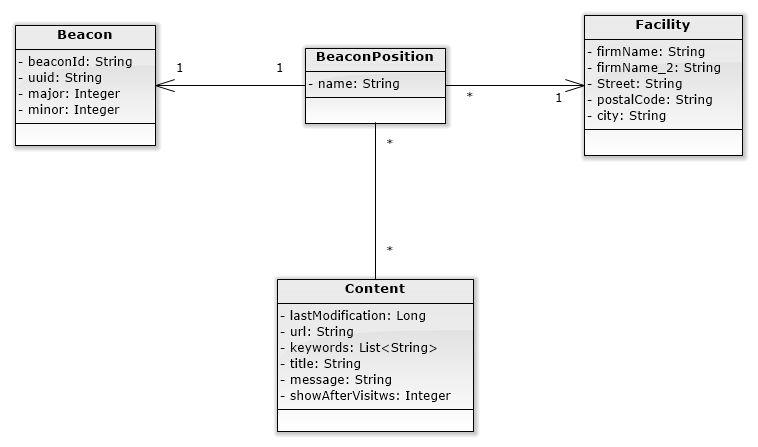
\includegraphics[scale=0.5]{./Abbildungen/Classdiagram1.png}
\label{fig:classdiagram}
\end{figure}
\end{frame}

\begin{frame}[fragile]
\frametitle<presentation>{Schnittstellenvereinbarung}


\begin{lstlisting}[language=Java, basicstyle=\ttfamily\scriptsize]
public interface IBeaconPositionProvider {

  public BeaconPosition getBeaconPositionForBeaconProps(
    String uuid,
    Integer major,
    Integer minor);
	
}

\end{lstlisting}


\end{frame}

% Implementierung


\section{Implementierung}

\begin{frame}
\frametitle{Datenbankschema}

\begin{figure}[!h]
\centering
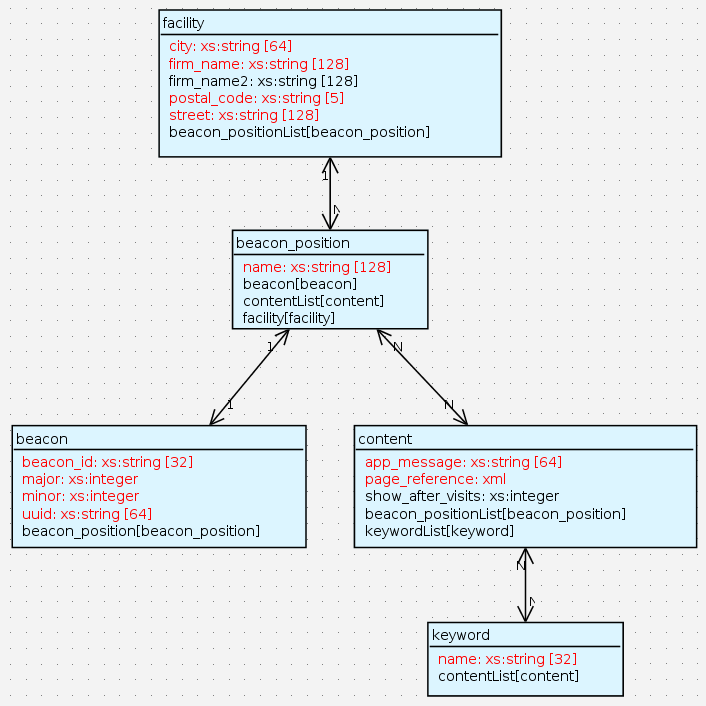
\includegraphics[scale=0.27]{./Abbildungen/dbschema.png}
\label{fig:dbschema-fs-beacon}
\end{figure}

\end{frame}

\begin{frame}[fragile]
\frametitle{Formular}
\framesubtitle{Tabellenvorlage Beacon}

\begin{lstlisting}[language=XML, basicstyle=\ttfamily\scriptsize]
<CMS_INPUT_TEXT name="cs_uuid" allowEmpty="no" 
    hFill="yes" singleLine="no" useLanguages="no">
    <LANGINFOS>
      <LANGINFO lang="*" label="UUID"/>
    </LANGINFOS>
</CMS_INPUT_TEXT>
	
<CMS_INPUT_NUMBER name="cs_major" allowEmpty="no" 
    hFill="yes" noBreak="yes" singleLine="no" 
    useLanguages="no">
    <LANGINFOS>
      <LANGINFO lang="*" label="Major" format="#"/>
    </LANGINFOS>
</CMS_INPUT_NUMBER>
\end{lstlisting}

\end{frame}

\begin{frame}
\frametitle{Mapping}
\framesubtitle{Tabellenvorlage Beacon}

\begin{figure}[!h]
\centering
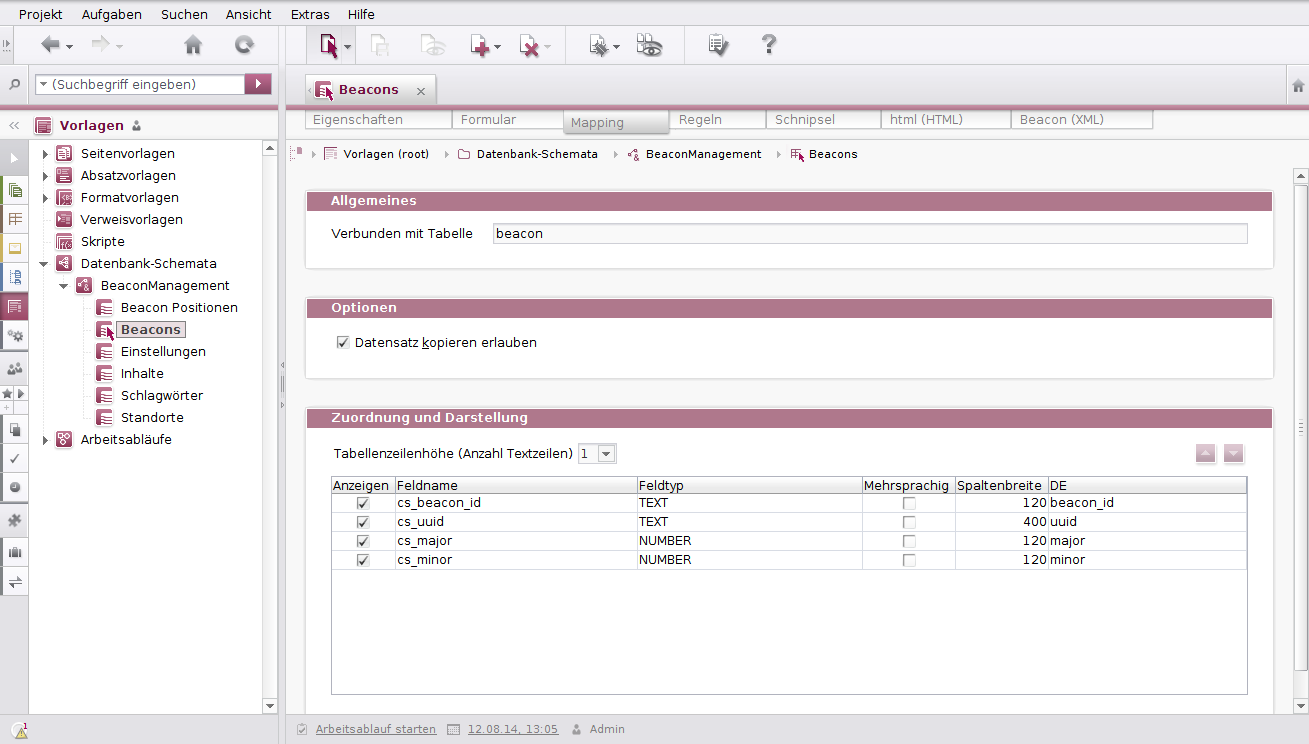
\includegraphics[scale=0.24]{./Abbildungen/mapping-table-beacon.png}
\end{figure}

\end{frame}

\begin{frame}[fragile]
\frametitle{Regeln}
\framesubtitle{Tabellenvorlage Beacon}

\begin{lstlisting}[language=XML, basicstyle=\ttfamily\scriptsize]
<ON_SAVE>
  <IF><NOT>
    <PROPERTY source="cs_uuid" name="EMPTY"/>
  </NOT></IF>
  <WITH>
    <MATCHES regex="^[0-9a-f]{8}-([0-9a-f]{4}-){3}" + 
      "[0-9a-f]{12}$">
      <PROPERTY source="cs_uuid" name="VALUE"/>
    </MATCHES>
  </WITH>
  <DO><VALIDATION>
    <PROPERTY source="cs_uuid" name="VALID"/>
    <MESSAGE lang="*" text="Invalid UUID"/>
    <MESSAGE lang="DE" text="Ungültige UUID"/>
  </VALIDATION></DO>
</ON_SAVE>
\end{lstlisting}

\end{frame}

\begin{frame}[fragile]
\frametitle{Ausgabekanal (XML)}
\framesubtitle{Tabellenvorlage Content}

\begin{lstlisting}[language=xml, basicstyle=\ttfamily\scriptsize] 
<content fs_id="$CMS_VALUE(#row.getId())$"> 
  [...]
  <relative_url>$CMS_REF(#row.page_reference, 
    templateSet:"html", abs:0)$
  </relative_url>
  <keywords>
    $CMS_IF(!#row.keywordList.isEmpty)$
      $CMS_FOR(_keyword, #row.keywordList)$
        <keyword>$CMS_VALUE(_keyword.name)$</keyword>
      $CMS_END_FOR$
    $CMS_END_IF$
  </keywords>
  <last_modification>$CMS_VALUE(#row.page_reference
    .getPageRef().getPage().getLastChanged())$
  </last_modification>
  [...]
</content>
\end{lstlisting}

\end{frame}



\begin{frame}
\frametitle{Schnittstelle zur Personalisierungskomponente}

\begin{itemize}
  \item Erstellung von Datenbank-Sichten (Views)
  \item DAO-Klassen (Spring JDBC-Schablonen)
\end{itemize}  
  
  \textbf{Problem}
  \begin{itemize}
  \item kein Zugriff auf FirstSpirits interne Datenbank
  \end{itemize}
  
\textbf{Lösung}
  \begin{itemize}
    \item XML-Export auf Webserver bei Veröffentlichung
  \begin{itemize}
    \item Kopplung an Veröffentlichungsprozess
    \item Performance $\Rightarrow$ Caching
    \end{itemize}
\end{itemize}

\end{frame}

\begin{frame}[fragile]
\frametitle{Http-HEAD}
\framesubtitle{Http-Antwort auf eine HEAD-Anfrage}

\begin{lstlisting}[basicstyle=\ttfamily\scriptsize] 
HTTP/1.1 200 OK
...
Date: Fri, 29 Aug 2014 16:11:59 GMT
Content-Type: text/xml; charset=UTF-8
Last-Modified: Thu, 28 Aug 2014 18:55:01 GMT
Content-Length: 6514
Server: Apache/2.2.12 (Unix)
Connection: close
...
\end{lstlisting}

\end{frame}

\begin{frame}
\frametitle{Caching}

\begin{figure}[!h]
\centering
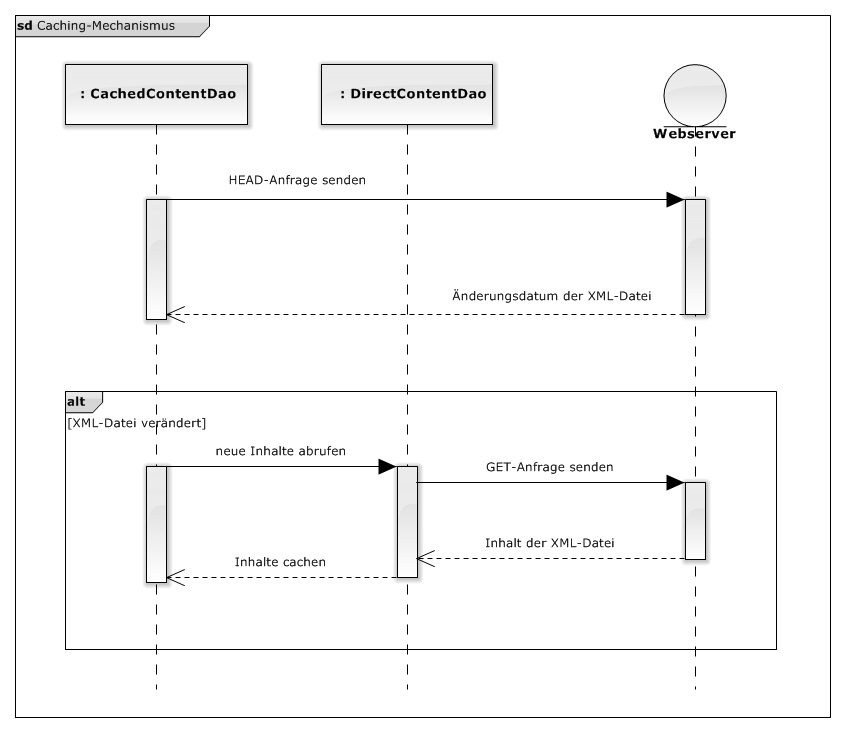
\includegraphics[scale=0.38]{./Abbildungen/Diagram2.png}
\label{fig:sequendiagramm}
\end{figure}

\end{frame}

\begin{frame}
\frametitle{Verwendete Java-Technologien}

\textbf{Frameworks und Bibliotheken}
\begin{itemize}
  \item Spring Core (Dependency Injection)
  \item Spring JDBC
  \item Spring OXM (JAXB)
  \item Apache HttpClient
  \item SLF4J / Log4j
\end{itemize}

\vskip0pt plus.5fill

\textbf{Software-Patterns}
\begin{itemize}
  \item Data Access Object (DAO)
  \item Singleton
  \item Factory
  \item Delegation
\end{itemize}


\end{frame}

% Fazit

\section[Fazit]{Fazit}

\begin{frame}
\frametitle<presentation>{Fazit}

{\textbf{Zusammenfassung}}

\begin{itemize}
\item Verwaltung von Beacons über FirstSpirit
\item Verknüpfung von Beacons mit Inhalten über FirstSpirit
\item Verfügbarmachung o.~g. Daten für Inhaltspersonalarisierung
\item Bereitstellung von ortsabhängigen und personalisierten
Inhalten aus FirstSpirit heraus (Gesamtsystem)
\end{itemize}

\vskip0pt plus.5fill

{\textbf{Ausblick}}

\begin{itemize}
\item Nutzung und Erweiterung sehr wahrscheinlich
\begin{itemize}
\item wachsende Informationsmenge im Web
\item verstärktes Kundeninteresse und Anfragen bei adesso
\item Präsentation auf Kundenveranstaltungen
\end{itemize}
\item Verbesserung des Caching-Mechanismus
\end{itemize}

\end{frame}

\end{document}


